\chapter{Технологический раздел}
В этом разделе приводится выбор языка программирования и средства программирования и рассматриваются необходимые библиотеки, которые используются для разработки программного обеспечения. Также описывается формат входных и выходных данных. Также приводятся описание пользовательского интерфейса и руководство пользователя для установки и использования программного обеспечения.
\section{Выбор средств реализации программного обеспечения}
\subsection{Выбор языка программирования}
Для реализации программного обеспечения был использован язык программирования Python\cite{python}. Этот выбор обусловлен следующими причинами:
\begin{itemize}[label = ---]
    \item это язык программирования высокого уровня, имеет простой синтаксис;
    \item наличие библиотек с открытым исходным кодом, позволяющих работать с естественным языком, выпонять классификации методом SVM и визуализировать данные;
    \item имеется навыки использования данного языка программирования, что сократить время написания программы.
\end{itemize}

\subsection{Выбор среды программирования}
Для разработки программы использовалась среда Visual Studio Code \cite{vscode} в качестве среды разработки по следующим причинам:
\begin{itemize}[label = ---]
    \item доступна бесплатная версия;
    \item имеет множество утилит, упрощающих написание кода;
    \item имеется навыки программирования при помощью данной среды, что сократить время написания программы.
\end{itemize}

Библиотека scikit-learn используется для работы с машинным обучением, потому что она предоставляет множество различных инструментов для разных задач машинного обучения, включая кластеризацию, регрессию, кластеризацию, обучение и тестирование моделей, а также предварительную обработку данных, и так далее. 

Для создания пользовательского интерфейса используется фреймворк Qt c помощью библиотеки PyQt5. Кроме того, в процессе разработки программного обеспечения библиотека pandas также используется для анализа набора данных, а библиотеки nltk и pymorphy2 — для очистки и предварительной обработки текстов.

\section{Формат входных и выходных данных}
Для модуля создания выборки данных входными данными является набор данных, скачанный с сайта kaggle.com, а выходные данные представляют собой файлы с указанным количеством строк для каждой темы.

На этапе обучения модели входными данными является файл, который создается из набора новостных текстов, в формате файла CSV. Каждая строка соответствует новости, состоящему из двух частей: текста и тематика новости. Каждый файл содержит определенное количество текста по каждой тематику.

На этапе классификации входными данными является текст или текстовый файл (в формате файла TXT), содержащий текст. Текст должен быть на русском языке, не менее 10 слов.

Результатом модуля классификации является прогнозируемое название тематика входного текста или содержимого файла и выводятся на пользовательский интерфейс программного обеспечения.

\section{Руководство пользователя}

Для запуска разработанного программного обеспечения требуется установить интерпретатор для Python и используемые библиотеки. Используемые в разработке библиотеки, которые необходимы для запуска ПО, приведены в файле requirements.txt, который находится в корневом каталоге проекта. С помощью пакетного менеджера pip все зависимости можно установить или обновить, запустив в терминале команду, приведенную в листинге \ref{lst:library}.

\begin{lstlisting}[caption=Установка всех необходимых библиотек,label=lst:library]
pip install -r requirements.txt
\end{lstlisting}

Для работы библиотеки nltk необходимо скачать библиотеки. Для установки библиотеки nltk и скачивания библиотек нужно в коде программы выполнить команды, приведенные в листинге \ref{lst:nltk}

\begin{lstlisting}[caption=Установка словарей nltk, label=lst:nltk]
import nltk
nltk.download()
\end{lstlisting}

Для создания выборки необходимо разместить папку с файлом исходного набора данных внутри корневого каталога проекта и запустить скрипт dataset.py. Скрипт может запущен из графического интерфейса среды разработки, либо командой из терминала, приведенную в листинге \ref{lst:data}.

\begin{lstlisting}[caption= Команда для создания обучающих выборок, label=lst:data]
python dataset.py
\end{lstlisting}

Чтобы обучить модель на заранее созданных размеченных выборках и предсказать тематик входного текста или текстового файла, пользователь может воспользоваться графическим интерфейсом приложения. Для открытия приложения необходимо запустить скрипт main.py посредством интерфейса среды разработки или командой в терминале, приведенную в листинге \ref{lst:run}.

\begin{lstlisting}[caption=Команда для запуска приложения, label=lst:run]
python main.py
\end{lstlisting}

В результате разработанное программное обеспечение может установить тематик текста или выдвинуть предположение, что может быть тематикой.

\section{Интерфейс пользователя}
Пользовательский интерфейс, который представлен на рисунке \ref{1-program}, был разработан с помощью программы Qt Designer. Интеграция с кодом на Python осуществлена посредством с помощью библиотеки PyQt5, которая предоставляет различные классы для работы с объектами пользовательского интерфейса.

\captionsetup{justification=centering,singlelinecheck=off}
\begin{figure}[h!]
	\centering
		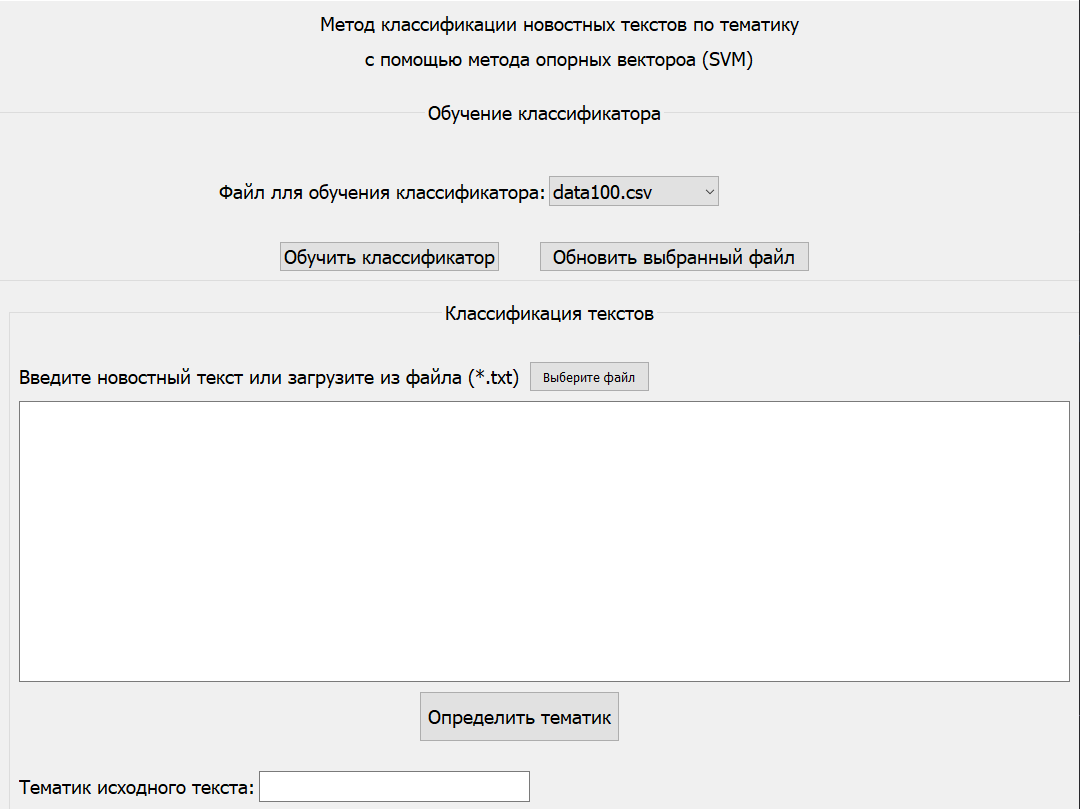
\includegraphics[,scale=0.55]{./img/1.png}
		\caption{Пользовательского интерфейса ПО}  
		\label{1-program}
\end{figure}
\newpage
Пользовательский интерфейс программного обеспечения состоит из 2 частей. В верхней части находится функционал обучения модели. В этом окне пользователь может выбрать файл для обучения модели из поля выбора. Каждый файл содержит определенное количество текста по каждой тематику. Пользователь может обновить содержимое этих файлов с помощью кнопки «Обновить выбранного файла». При нажатии на кнопку «Обучить модель» выбранная выборка разбивается на две части: 80\% корпуса –-- обучающая выборка, 20\% --– тестовая. Программа сообщит, когда модель завершит обучение , как показано на рисунке \ref{3-program}.

\captionsetup{justification=centering,singlelinecheck=off}
\begin{figure}[h!]
	\centering
		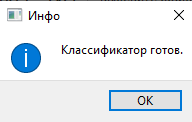
\includegraphics[,scale=1.5]{./img/3.png}
		\caption{Модель готова}  
		\label{3-program}
\end{figure}
\newpage
В нижней части находится функционал предсказания тематика текста. Если пользователь попытается определить тематик, не обучив сначала модель, будет возвращена ошибка, как показано на рисунке \ref{2-program}.

\captionsetup{justification=centering,singlelinecheck=off}
\begin{figure}[h!]
	\centering
		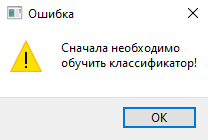
\includegraphics[,scale=1.55]{./img/2.png}
		\caption{Ошибка, возникающая в случае, если модель не обучена}  
		\label{2-program}
\end{figure}

Пользователь может ввести текст в поле ввода или выбрать файл. Программа поддерживает только txt файлы (текстовые файлы). При нажатии на кнопку «Выбрать файл» открывается файловая система компьютера, в которой необходимо выбрать интересующий текстовый файл. Когда пользователь выбирает файл, его содержимое отображается в текстовом поле. Если пользователь нажимает кнопку «Определить тематик», когда вводимый текст пуст или имеет неверный формат, будет возвращена ошибка, как показано на рисунке \ref{4-program}.

\captionsetup{justification=centering,singlelinecheck=off}
\begin{figure}[h!]
	\centering
		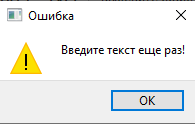
\includegraphics[,scale=1.5]{./img/4.png}
		\caption{Ошибка, возникающая в случае, если текстовое поле пусто}  
		\label{4-program}
\end{figure}
\newpage
Если входной текст не пуст, то запускается алгоритм классификации. После того, как модель завершит работать, на экран будет выведено название наиболее вероятного тематика, как показано на рисунке \ref{5-program}.

\captionsetup{justification=centering,singlelinecheck=off}
\begin{figure}[h!]
	\centering
		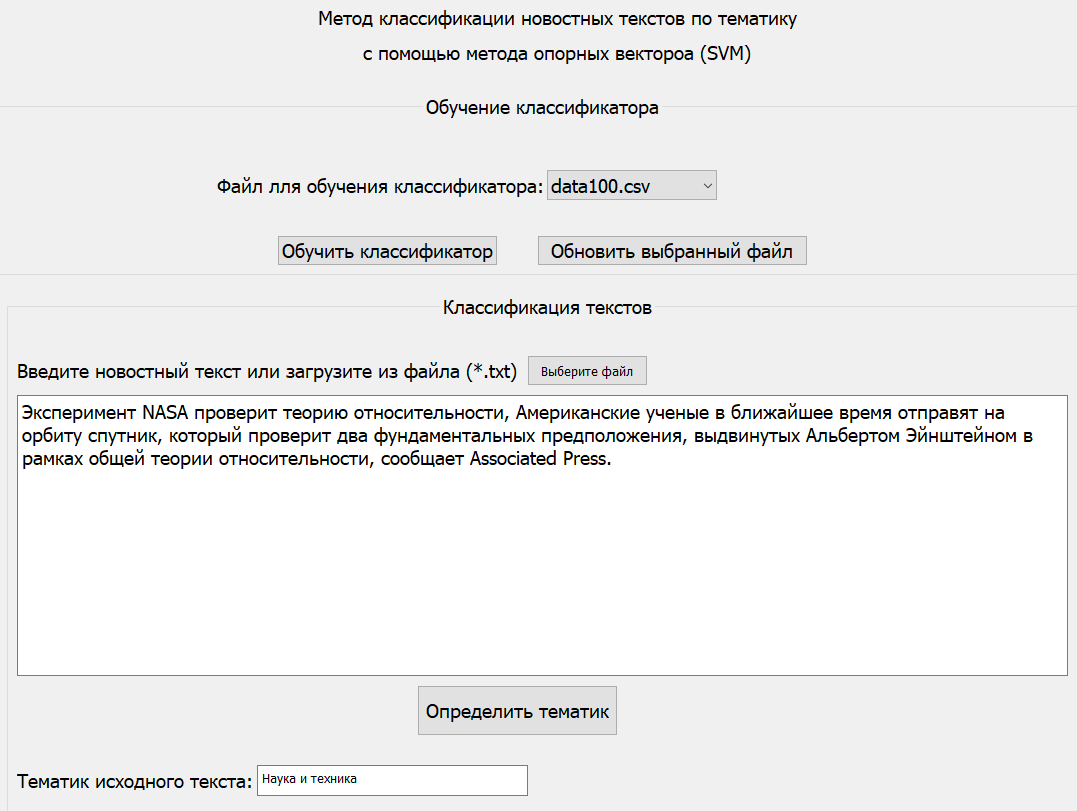
\includegraphics[,scale=0.55]{./img/5.png}
		\caption{Результат работы классификации}  
		\label{5-program}
\end{figure}

\section*{Вывод}
В этом разделе были приведены выбор языка программирования и средства программирования и рассмотрены необходимые библиотеки, которые используются для разработки программного обеспечения. Также был описан формат входных и выходных данных. Также были приведены описание пользовательского интерфейса и руководство пользователя для установки и использования программного обеспечения.